\hypertarget{dockarchived_8cpp}{}\section{O\+L13/dockarchived.cpp File Reference}
\label{dockarchived_8cpp}\index{O\+L13/dockarchived.\+cpp@{O\+L13/dockarchived.\+cpp}}


Fenetre dialoque permettant l\textquotesingle{}edition d\textquotesingle{}une nouvelle note.  


{\ttfamily \#include \char`\"{}dockarchived.\+h\char`\"{}}\newline
{\ttfamily \#include \char`\"{}ui\+\_\+dockarchived.\+h\char`\"{}}\newline
Include dependency graph for dockarchived.\+cpp\+:\nopagebreak
\begin{figure}[H]
\begin{center}
\leavevmode
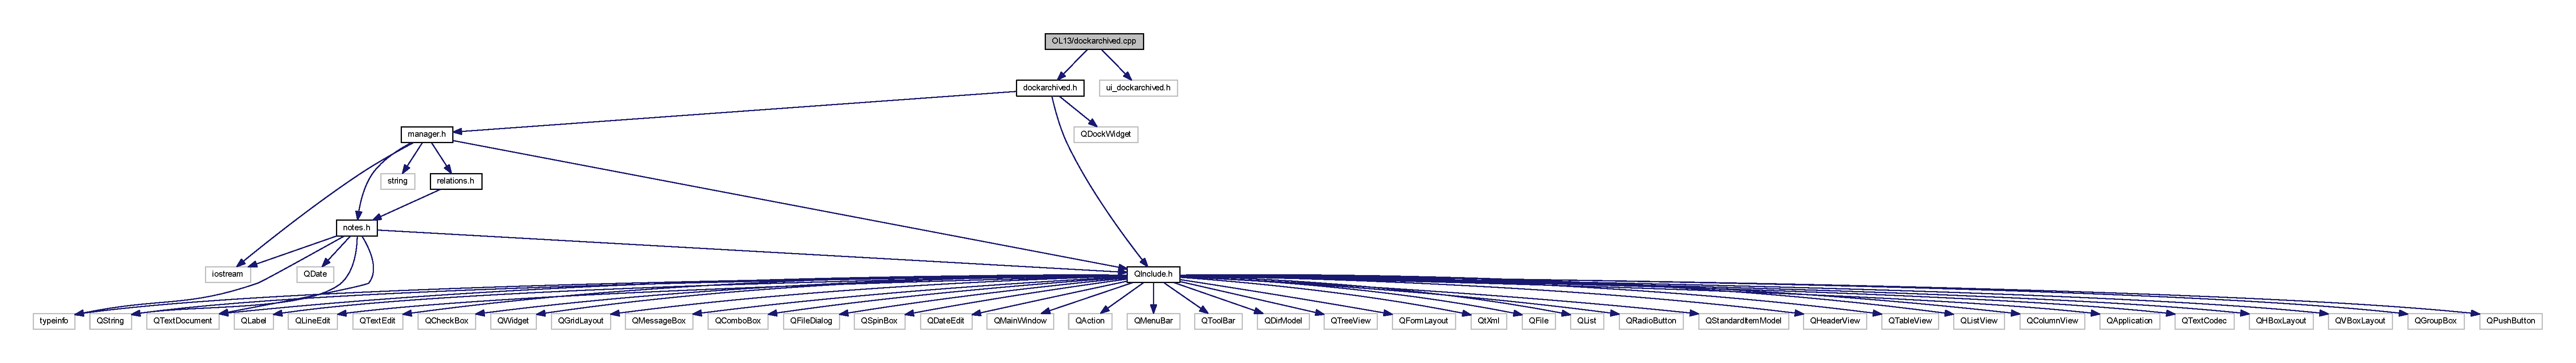
\includegraphics[width=350pt]{dockarchived_8cpp__incl}
\end{center}
\end{figure}


\subsection{Detailed Description}
Fenetre dialoque permettant l\textquotesingle{}edition d\textquotesingle{}une nouvelle note. 

\begin{DoxyAuthor}{Author}
Garnier Maxime, Naudin Louise, Pépin Hugues 
\end{DoxyAuthor}
\begin{DoxyVersion}{Version}
1.\+0 
\end{DoxyVersion}
\begin{DoxyDate}{Date}
14 Juin 2017
\end{DoxyDate}
class \+:
\begin{DoxyItemize}
\item \hyperlink{class_dock}{Dock}\+:classe abstraite
\item \hyperlink{class_dock_remove}{Dock\+Remove}
\item \hyperlink{class_dock_archived}{Dock\+Archived} \begin{DoxyVerb}  Attribut:
          QNote note
  Signaux :
          change_creer() signal interne à la fenetre.
          NewNote() envoie la note créer à l'interface //Plus utile.\end{DoxyVerb}

\end{DoxyItemize}